\documentclass[lettersize,journal]{IEEEtran}

\usepackage{amsmath,amssymb}
%\usepackage[UTF8]{ctex}
\usepackage{graphicx}
\graphicspath{{figures/}}
\usepackage{booktabs}
\usepackage{array}
\usepackage{multirow}
\usepackage{url}
\usepackage{xcolor}
\usepackage{orcidlink}

\usepackage[ruled,linesnumbered]{algorithm2e}
% 子图命令：图片上方自动编号 (a),(b),(c)...
\newcounter{subfigcnt}[figure]
\renewcommand{\thesubfigcnt}{(\alph{subfigcnt})}
\newcommand{\subimg}[1]{%
  \refstepcounter{subfigcnt}%
  \begin{minipage}[t]{0.32\textwidth}\centering
  \includegraphics[width=\linewidth]{#1}\\[2pt]
  \footnotesize\thesubfigcnt
  \end{minipage}}%
\newcommand{\subimgw}[1]{%
  \refstepcounter{subfigcnt}%
  \begin{minipage}[t]{0.48\textwidth}\centering
  \includegraphics[width=\linewidth]{#1}\\[2pt]
  \footnotesize\thesubfigcnt
  \end{minipage}}%

\title{QoS-FiLM: Intent-Conditioned GNNs for Per-Flow QoS Routing}

\author{Xiaolong Cui\textsuperscript{*}\hspace{-1.5mm}$^{~\orcidlink{0009-0008-1615-6727}}$, Yuwei Deng\textsuperscript{*}, Zixu Wang, Xiying Fan, Wei Huangfu\textsuperscript{\textdagger}\hspace{-1.5mm}$^{~\orcidlink{0000-0003-2887-8395}}$, ~\IEEEmembership{Senior Member,~IEEE}
\thanks{\textsuperscript{*}These authors contributed equally to this work.}
\thanks{Supported in part by the National Key Research and Development Program under grant 2023YFB2903901.
The authors are with the School of Computer and Communication Engineering, University of Science and Technology Beijing, Beijing 100083, China (e-mail: cuixl@ustb.edu.cn). 
\textsuperscript{\textdagger}Corresponding author: Wei Huangfu.}
}
\begin{document}
\bstctlcite{IEEEexample:BSTcontrol}
\maketitle

\begin{abstract}
Modern backbone networks carry heterogeneous traffic: small-bandwidth flows (e.g., latency-sensitive control signaling, interactive web) demand strict latency guarantees and full bandwidth satisfaction, whereas large-bandwidth flows (e.g., distributed AI training, bulk backup) prioritize maximizing throughput and accept best-effort service. Existing online routing heuristics are myopic because they cannot foresee future arrivals. Recent learning-based methods address the myopia problem yet still suffer from a critical limitation: they produce a single topology embedding shared by all flows regardless of the QoS intent, thereby limiting their ability to differentiate routing under mixed services. We present QoS-FiLM, a flow-conditioned graph architecture that uses Feature-wise Linear Modulation (FiLM) to inject the QoS intent of each flow into every message-passing layer of a Graph Neural Network (GNN). This enables the same substrate graph to yield distinct embeddings for heterogeneous flows. We cast online per-flow routing as a stochastic Markov decision process and train the policy with proximal policy optimization (PPO). Across the GEANT, NOBEL-EU, and ABILENE topologies, QoS-FiLM surpasses both classical heuristics and learned network baselines in cumulative utility, bandwidth satisfaction ratio, and end-to-end latency. On GEANT, it improves the mean reward by $0.219$ over the flow-unaware baseline noFiLM-Tf, with bandwidth score improvements of $26.3\%$ and average delay reductions of $28.5\%$. Ablation studies confirm the essential role of FiLM conditioning and its strong synergy with the attention mechanism, while interpretability analysis verifies the high sensitivity of the encoder to QoS intent and the differentiation of routing decisions by flow type.
\end{abstract}

\begin{IEEEkeywords}
online routing, graph neural networks, QoS differentiation, feature-wise linear modulation, deep reinforcement learning
\end{IEEEkeywords}

% ===== English Sections =====
\section{Introduction}
\label{sec:intro}

Traffic heterogeneity has become a central challenge for backbone networks. The same infrastructure must simultaneously carry interactive video, remote control, distributed AI training, and bulk backup, and these services differ sharply in their preferences for bandwidth, latency, and packet loss across multiple QoS dimensions. The result is a coexistence of mouse flows (low bandwidth, strict QoS requirements) and elephant flows (high bandwidth, best-effort tolerant)~\cite{CISCO2023_GlobalTraffic}. Such heterogeneous demand leaves traditional undifferentiated routing strategies, whether shortest-hop-count OSPF or equal-cost multipath ECMP, unable to satisfy resource utilization and QoS guarantees at the same time.

The fundamental difficulty lies in an online causal coupling: flows arrive sequentially, and the future is unseen. When selecting a route for the $t$-th flow, the agent cannot foresee the subsequent demands $\mathbf{f}_{t+1}, \dots, \mathbf{f}_W$~\cite{Wang1996_QoSRouting}. Were the entire flow sequence available offline, route selection could be cast as an integer program with a globally optimal solution; the online constraint, however, forces decisions under incomplete information, so that earlier and later flows compete for shared link capacity. Greedy heuristics such as CSPF, though locally optimal at each step, frequently place early-arriving mouse flows on resource-rich optimal paths and thereby deplete the link capacity later needed by elephant flows, a classic dilemma of myopic strategies~\cite{Fortz2000_TrafficEngineering}. An optimal policy must instead reserve capacity non-myopically in expectation over the demand distribution, trade off across flows, and attribute the cumulative utility realized at the end of the sequence back to earlier steps. This structure, sequential decision-making under an unseen future with long-range credit assignment, is naturally suited to reinforcement learning (RL).

Combining deep reinforcement learning (DRL) with graph neural networks (GNNs) has opened new possibilities for online routing: DRL supplies non-myopic sequential decision-making~\cite{Sun2022_ScalableRouting_TON,He2024_RoutingOptimization_TMC}, and GNNs provide explicit encoding of network topology~\cite{Rusek2020_JSAC_RouteNet,FerriolGalmes_2023_RouteNetFermi,Munikoti2024_DRL_GNN_TNNLS}. Existing methods nonetheless suffer from two fundamental limitations. First, DRL routing policies typically optimize a single global objective for all flows and cannot provide differentiated service under mixed traffic. Second, GNN-based methods learn one unified topology embedding for all flows and cannot tailor that embedding to per-flow QoS characteristics, the ``same graph, same embedding'' problem.

Breaking this homogeneity constraint requires a network encoder with flow-conditioning capability: it must adjust its topological perception dynamically according to each flow's individual QoS characteristics. Conditioned neural networks, such as FiLM for general networks~\cite{Perez2018_FiLM} and its graph extension GNN-FiLM~\cite{Brockschmidt2020_GNNFiLM}, supply the necessary mechanisms, yet they have not been applied to per-flow QoS-aware routing. In the online routing scenario, what truly needs conditioning is not intra-graph node attributes but per-flow QoS intent: the same topology, when facing a mouse flow versus an elephant flow, should undergo a message-passing process reshaped into two entirely different topological perceptions. No prior work has brought FiLM conditioning into per-flow online routing, leaving differentiated topology perception and policy learning under mixed traffic an open problem.

To close this gap, we propose QoS-FiLM. The core idea is to inject the QoS intent vector of each flow into every message-passing layer of a GNN via FiLM, so that the same physical topology is encoded into differentiated node embeddings under different intents. We then formalize online mixed-service routing as a Markov decision process (MDP) and train a non-myopic routing policy with proximal policy optimization (PPO). The main contributions of this paper are as follows:
\begin{itemize}
    \item \textbf{A flow-aware graph reinforcement learning architecture for mixed-service online routing.}
    The architecture couples a flow-conditioned graph encoder, a path-aware scorer, and an independent value network, all trained end-to-end via proximal policy optimization. It resolves the core contradiction that the same topology must yield differentiated routing decisions for flows with different QoS intents.

    \item \textbf{A per-flow QoS-intent-driven FiLM conditioning mechanism and network design.}
    The per-flow intent vector generates affine modulation parameters for each GNN layer, rendering the message-passing process flow-aware. We further design complementary modules, including LSTM-based path embedding pooling, intent-path joint scoring, and intent-conditioned attention graph pooling, which together realize a complete flow-conditioned decision chain from topology encoding to path selection.

    \item \textbf{Dual-space interpretability validation.}
    Experiments show that the proposed architecture significantly outperforms classical baselines in cumulative utility, bandwidth satisfaction ratio, and end-to-end latency. A dual-space analysis in the representation space (hidden feature separability) and the decision space (path selection differentiation) further confirms that merely changing the QoS intent triggers differentiated routing decisions on the same topology and the same source-destination node pair, validating the necessity of FiLM conditioning at the mechanism level.
\end{itemize}

The remainder of this paper is organized as follows. Section~II reviews related work on online routing and conditioned graph representation learning. Section~III formalizes online mixed-service routing as a Markov decision process and defines the optimization objective. Section~IV details the QoS-FiLM architecture, including the flow-conditioned graph encoder, the path-aware scorer, the independent value network, and the per-layer FiLM conditioning mechanism. Section~V reports the experimental design, main results, ablation analysis, and interpretability validation on the GEANT, NOBEL-EU, and ABILENE backbone topologies. Section~VI concludes the paper and outlines future work.

\section{Related Work}
\label{sec:related}

This section surveys recent research across four dimensions: traditional QoS routing, DRL-based routing, GNN-based network modeling, and graph network conditioning mechanisms.

\subsection{Traditional QoS Routing and Traffic Engineering}

Classical mechanisms such as OSPF, ECMP, and CSPF perform hop-by-hop forwarding based on static link weights and lack differentiated service capability under mixed traffic scenarios. Wang and Crowcroft established the constraint optimization framework for QoS routing~\cite{Wang1996_QoSRouting}; Fortz and Thorup revealed the limitations of weight-optimization-based traffic engineering under dynamic demand~\cite{Fortz2000_TrafficEngineering}. Brundiers et al.\ studied the benefits of loops in Segment Routing for traffic engineering, demonstrating the potential of flexible path control in dynamic load balancing~\cite{Brundiers2021_Loops_SR_TE}, and further proposed a midpoint optimization approach for finer-grained traffic engineering control~\cite{Brundiers2022_Midpoint_SR_INFOCOM}\textcolor{red}{这篇文献编译出来还是不对，check一下，找了一下原因，因为有另外一篇文献跟这个作者相同，所以被省略了，找下解决方案}. The common shortcoming of these methods lies in their myopia: each decision is independently optimized and cannot reserve resources for heterogeneous flows from a global network perspective or a long-term sequential view. When mouse flows and elephant flows share links, static strategies often fail to simultaneously satisfy strict latency guarantees and high throughput.

\subsection{DRL-Based Network Routing}

To overcome the limitations of fixed rules, researchers have introduced DRL into routing decisions. Liu et al.\ proposed DRL-OR, using multi-objective DRL to handle heterogeneous service demands~\cite{Liu2021_DRLOr_INFOCOM}. Casas-Velasco et al.\ proposed DRSIR, achieving intelligent routing decisions in SDN via deep Q-learning~\cite{CasasVelasco2021_DRSIR_TNSM}. Chen et al.\ proposed an adaptive multipath routing optimization framework based on multi-agent meta-reinforcement learning~\cite{Chen2022_MultiagentMeta_TNNLS}. Suzuki et al.\ proposed a multi-agent deep reinforcement learning method for jointly optimizing computation offloading and routing decisions in multi-cloud edge networks, validating the adaptive capability of multi-agent collaboration in dynamic network environments~\cite{Suzuki2023_MADRL_Routing_TNSM}. Sanchez et al.\ proposed DQS, achieving routing optimization in SDN via QoS-driven DRL~\cite{Sanchez2024_DQS_JPDC}. However, the above methods share two common limitations. First, their policy networks mostly encode network state via fully connected layers or simple embeddings, lacking explicit modeling of topological structure and thus suffering from limited generalization. Second, they typically optimize a single global objective for all flows (e.g., minimizing maximum link utilization or average latency) without embedding per-flow QoS intent as a conditioning signal into the policy network, and therefore cannot achieve differentiated routing under mixed traffic.

\subsection{GNN-Based Network Modeling and Routing}

GNNs provide a natural tool for encoding network topology, with existing research proceeding along two directions.

The first is offline performance modeling. Rusek et al.\ proposed RouteNet~\cite{Rusek2020_JSAC_RouteNet} and Ferriol-Galm\'{e}s et al.\ proposed RouteNet-Fermi~\cite{FerriolGalmes_2023_RouteNetFermi}, using message-passing neural networks to predict link delay and packet loss. Huang et al.\ proposed xNet, achieving flow-level QoS prediction by learning temporal state transitions~\cite{Huang2024_ToN_xNetModeling}. These methods focus on offline modeling under aggregated traffic, learning ``one graph, one global embedding,'' and cannot adapt to online per-flow decisions.

The second is graph-aware policies for online decision-making. Almasan et al.\ validated the improvement in routing quality from the joint application of GNNs and DRL~\cite{Almasan2022_RLmeetsGNN}; Bern\'{a}rdez et al.\ proposed MAGNNETO, a multi-agent GNN system for distributed traffic engineering~\cite{Bernardez2023_MAGNNETO_TCCN}; Yang et al.\ and Dong et al.\ respectively explored graph-aware joint optimization of routing and scheduling in time-sensitive networking and network slicing scenarios~\cite{Yang2022_GCN_RL_IoTJ,Dong2022_GCN_Slicing_Routing_TCCN}; Bhuvanasi et al.\ achieved resilient routing using GNNs and multi-agent DRL~\cite{Bhuvanasi2023_ResilientRouting_TNSM}. Although these methods introduce GNNs into online decision-making, they still produce a unified topological representation for all flows. When mouse flows and elephant flows arrive sequentially, the system sees the same embedding of the same graph, unable to perform differentiated perception based on per-flow QoS characteristics, let alone make different routing decisions accordingly. Collectively, these methods constitute the paradigm that couples GNN topology encoding with DRL path selection. The absence of flow conditioning makes this paradigm a natural but undifferentiated baseline.

\subsection{Conditioning Mechanisms for GNNs}

To enable network representations to dynamically adjust according to external conditions, researchers have proposed various conditioning mechanisms. These mechanisms can be classified by the level at which the conditioning signal operates into three categories:
(1)~\textbf{Node-level conditioning}, such as GNN-FiLM proposed by Brockschmidt et al.~\cite{Brockschmidt2020_GNNFiLM}, which generates affine modulation parameters from target node features to directly reshape the message-passing process; (2)~\textbf{Edge-level dynamic weights}, such as GATv2 by Brody et al.~\cite{Brody2022_GATv2}, which computes adaptive attention weights via dynamic interaction of node features, achieving conditioned adjustment of relational strength; (3)~\textbf{Type-level conditioning}, such as the Heterogeneous Graph Transformer by Hu et al.~\cite{Hu2020_HGT}, which uses node type as a semantic condition to differentiate feature transformations across different relation patterns.

However, the conditioning signals in the above mechanisms all originate from intra-graph structure (target nodes, edge features, node categories, etc.), rather than from per-flow external QoS intent. In the online routing scenario, what distinguishes embeddings is the QoS characteristics of the arriving flow: the same topology, when facing a mouse flow versus an elephant flow, should produce markedly different node representations and routing decisions. No prior work has introduced FiLM conditioning into the per-flow online routing scenario, and differentiated topology perception and policy learning remain open problems.

In summary, the existing literature exhibits clear gaps: (1)~traditional methods are myopic and cannot handle mixed QoS; (2)~DRL methods lack explicit topological modeling; (3)~GNN methods assume homogeneous traffic and suffer from the ``same graph, same embedding'' representational homogeneity problem; (4)~conditioned GNNs have not been applied to per-flow online routing. QoS-FiLM addresses these limitations.

\section{Problem Formulation}
\label{sec:problem}

We formulate the online per-flow routing problem as a stochastic optimization and show why it requires a reinforcement learning approach.

\subsection{Network and Traffic Model}
\label{sec:problem:model}

Consider a directed network $G=(V,E)$ with node set $V$ and link set $E$. Each link $e\in E$ has a delay $d_e$ and bandwidth capacity $c_e$; let the residual bandwidth at a given time be $b_e^{\text{res}}\in[0,c_e]$, with initial value $b_e^{\text{res}}=c_e$.

Traffic arrives online in \emph{sequences} (episodes): a sequence contains $W$ flows arriving sequentially. The agent selects a route for each flow immediately upon arrival and cannot foresee subsequent flows. Once a flow is assigned a path, it continuously occupies its bandwidth for the duration of the sequence -- the ``permanent connection / infinite holding time'' assumption of online routing; this paper does not model flow departures. After the sequence ends, capacities are reset and a new batch of arrivals begins.

The $t$-th flow is described by a quadruple $\mathbf{f}_t = (o_t,\, v_t,\, \phi_t,\, b_t), t=1,\dots,W $, where $o_t, v_t\in V$ are source and destination nodes, $b_t$ is the bandwidth demand, and $\phi_t\in[0,1]$ is the \emph{QoS intent coefficient}. $\phi_t$ follows a flipped Pareto distribution (parameter $\alpha$), with a heavy tail concentrated in the low-$\phi$ region, so that the overwhelming majority of flows are mouse flows with strict latency and bandwidth constraints, and only a small number are elephant flows with relaxed constraints. The bandwidth demand $b_t$ is derived from $\phi_t$ via a positively correlated linear mapping with Gaussian perturbation:
\begin{equation}
b_t = b_{\text{floor}} + (b_{\text{max}}-b_{\text{floor}})\cdot\phi_t + \mathcal{N}(0,\sigma),
\label{eq:bw_gen}
\end{equation}
so that $\phi_t$ and $b_t$ are strongly positively correlated (Pearson $r\approx 0.90$) but not fully deterministic — $\phi_t$ still carries independent QoS information beyond $b_t$. Together, $(\phi_t, b_t)$ jointly characterize a flow: an elephant flow is ``large-volume and tolerant of best-effort delivery'', while a mouse flow is ``small-volume but requires strict guarantees''. Flow sequences are sampled from a demand distribution $\mathcal{D}$, i.e., $(\mathbf{f}_1,\dots,\mathbf{f}_W)\sim\mathcal{D}$.

When processing each flow, the system precomputes $K$ candidate shortest paths $\mathcal{P}_t=\{p_t^{1},\dots,p_t^{K}\}$ ($K$-shortest paths, hop-count-based). The routing decision is to assign one path $p_t\in\mathcal{P}_t$ from this candidate set to carry $\mathbf{f}_t$. Once assigned, the residual bandwidth of links along the path is reduced by the actual occupancy and is not released within the sequence, thereby changing the available capacity faced by subsequent arriving flows -- this is the resource competition between earlier and later flows: the capacity occupied by earlier flows reduces the feasible set of later flows.

\subsection{Service Quality Metrics}
\label{sec:problem:metrics}

Given the path $p_t$ selected for $\mathbf{f}_t$, we define the bandwidth satisfaction ratio and effective end-to-end delay as its service quality metrics.

\textbf{Bandwidth satisfaction ratio.} The bandwidth deliverable by the path is constrained by the bottleneck link. Define
\begin{equation}
\hat b_t = \min\!\Big(\min_{e\in p_t} b_e^{\text{res}},\; b_t\Big),
\qquad
\rho_t = \hat b_t/b_t,
\label{eq:rho}
\end{equation}
where $\rho_t\in[0,1]$ (since $\hat b_t\le b_t$ and $\hat b_t\ge 0$, the range is naturally bounded) is the bandwidth satisfaction ratio; $\rho_t=1$ indicates that the demand is fully satisfied.

\textbf{End-to-end effective delay.} We use a \emph{congestion-aware effective delay proxy} to characterize the impact of link occupancy on delay: the fuller the link, the higher the effective delay. Let the residual capacity ratio after occupancy be $u_e = b_e^{\text{res}}/c_e\in[0,1]$, and define the path effective delay as
\begin{equation}
\hat D_t = \sum_{e\in p_t}\big(1-\log u_e\big)\, d_e,
\label{eq:delay}
\end{equation}
where the physical propagation delay $d_e$ is multiplied by a congestion penalty factor $(1-\log u_e)$ that increases with occupancy: when idle ($u_e\!=\!1$) the factor is $1$ and the effective delay falls back to the physical delay; when fully loaded ($u_e\!\to\!0$) the factor diverges. Eq.~\eqref{eq:delay} is not a physical delay derived from queueing theory, but a log-barrier-style monotonic congestion cost — it pushes the policy away from fully loaded links. In RL it serves only as a reward shaping signal; its monotonicity (higher congestion $\Rightarrow$ higher cost), not its absolute value, drives policy learning. Compared with the classic M/M/1 queueing $1/(1-\rho)$ hyperbolic divergence, this proxy grows more slowly and applies a milder penalty to extreme congestion.

\subsection{Utility Function and Optimization Objective}
\label{sec:problem:objective}

The QoS intent $\phi_t$ determines what a flow ``cares about.'' We use $\phi_t$ to combine the bandwidth and delay metrics into a single per-flow utility:
\begin{equation}
\begin{split}
U(\mathbf{f}_t, p_t) &=
\underbrace{\big[(1-\phi_t)\,\mathbb{1}[\rho_t\!\ge\!1] + \phi_t\,\rho_t\big]}_{\text{bandwidth utility }U^{\text{bw}}_t} \\
&\quad +
\underbrace{(1-\phi_t)\,\frac{1}{1+\hat D_t/\tau}}_{\text{delay utility }U^{\text{dl}}_t},
\end{split}
\label{eq:utility}
\end{equation}
Eq.~\eqref{eq:utility} imposes fundamentally different objectives on the two types of flows:

\begin{itemize}
\item When $\phi_t\!\to\!0$ (mouse flow): the bandwidth utility reduces to a hard satisfaction indicator $\mathbb{1}[\rho_t\!\ge\!1]$ (scoring only when bandwidth is fully satisfied), and the delay utility weight attains its maximum -- i.e., requiring strict bandwidth guarantees and low latency.
\item When $\phi_t\!\to\!1$ (elephant flow): the bandwidth utility reduces to the continuous ratio $\rho_t$ (partial satisfaction also scores proportionally), and the delay utility term is switched off -- i.e., pursuing only throughput maximization.
\end{itemize}
where $\tau$ is a delay normalization constant (see Section~\ref{sec:exp:hyperparam} for the specific value).

\textbf{Optimization objective.} The routing policy must maximize the cumulative utility over the entire sequence in expectation over the demand distribution $\mathcal{D}$:
\begin{equation}
\max_{\{p_t\}}\;
\mathbb{E}_{(\mathbf{f}_1,\dots,\mathbf{f}_W)\sim\mathcal{D}}
\left[\sum_{t=1}^{W} U(\mathbf{f}_t, p_t)\right],
\label{eq:objective}
\end{equation}
where $\{p_t\}_{t=1}^{W}$ is the policy sequence of routing decisions at each step, and each $p_t\in\mathcal{P}_t$ is determined based only on current and historical observable information $\{\mathbf{f}_\tau, p_\tau\}_{\tau\le t}$ and the current network state under the online causal constraint, and \emph{cannot} depend on future flows $\{\mathbf{f}_\tau\}_{\tau>t}$ that have not yet arrived.

In Eq.~\eqref{eq:objective}, given a flow and a path, both the utility $U(\mathbf{f}_t,p_t)$ and the update of residual bandwidth are deterministic and computable, which might tempt one to think the problem can be solved via classical optimization or greedy rules. However, the true difficulty of this problem lies not in bookkeeping but in the \emph{unseen future}: flows arrive online sequentially, and when selecting a route for the $t$-th flow, the agent cannot foresee subsequent flows $\mathbf{f}_{t+1},\dots,\mathbf{f}_W$ (the online causal constraint). If the entire flow sequence were presented upfront, routing could certainly be formulated as an integer program to obtain a globally optimal solution; but such an offline optimum requires foreknowledge of the entire future, cannot be executed online, and can only serve as a post-hoc performance upper bound -- not to mention that the problem itself is NP-hard. Because the future is unseen, each current routing step alters the feasible set of subsequent flows via the residual bandwidth $b_e^{\text{res}}$: preferentially allocating mouse flows to low-latency, high-residual-bandwidth links may deplete the capacity later needed by elephant flows. Hence stepwise greedy approaches (e.g., CSPF, which selects the shortest constraint-satisfying path for each flow on arrival) are necessarily myopic. The optimal policy must, in expectation over the demand distribution $\mathcal{D}$, non-myopically reserve capacity and trade off across flows -- i.e., attribute the cumulative utility at the sequence end back to those earlier routing steps. This is exactly the structure that a Markov decision process captures. Section~\ref{sec:method} accordingly formalizes Eq.~\eqref{eq:objective} as an MDP and presents the solution method.

\label{sec:problem:why_rl}

\section{Methodology}
\label{sec:method}

We formalize the online routing optimization of Section~\ref{sec:problem:objective} as an MDP (\S\ref{sec:method:mdp}), justify the choice of PPO as the training algorithm (\S\ref{sec:method:algo}), and present the flow-aware QoS-FiLM architecture (\S\ref{sec:method:overview}--\ref{sec:method:train}). All network dimensions, layer counts, and training coefficients are written symbolically here; their specific values are listed in Section~\ref{sec:exp:hyperparam}.

\subsection{Architecture Overview}
\label{sec:method:overview}

Fig.~\ref{fig:film_gnn_arch} gives a high-level picture of the QoS-FiLM architecture, which consists of three main components. \textbf{(1) FiLM-GNN encoder:} takes as input the current graph snapshot (node and link features) and the flow intent vector $m_t = [\phi_t, \tilde b_t]$. At each graph attention layer, the intent vector generates per-channel scaling $\gamma^{(\ell)}$ and shifting $\beta^{(\ell)}$ parameters via lightweight MLPs; these modulate the message-passing output through an affine transformation $x^{(\ell)} = (1+\gamma^{(\ell)})\odot \tilde x^{(\ell)} + \beta^{(\ell)} + x^{(\ell-1)}$, so that the same physical topology yields different node embeddings for flows with distinct QoS requirements. \textbf{(2) Actor Head:} pools the node embeddings along each candidate path via an LSTM-based PathPooler, concatenates the resulting path representation with $m_t$, and scores the $K$ candidates through the KPathScorer to produce a Categorical action distribution. \textbf{(3) Critic Head:} aggregates the node embeddings into a graph-level vector via attention pooling (where attention weights depend on $m_t$) and regresses the state value $V_\psi(s_t)$ through an MLP. These three components operate in a closed MDP loop: the agent observes the current state, selects a path for the arriving flow, the environment updates link capacities, and PPO optimizes the policy from the collected trajectories.

\begin{figure}[t]
\centering
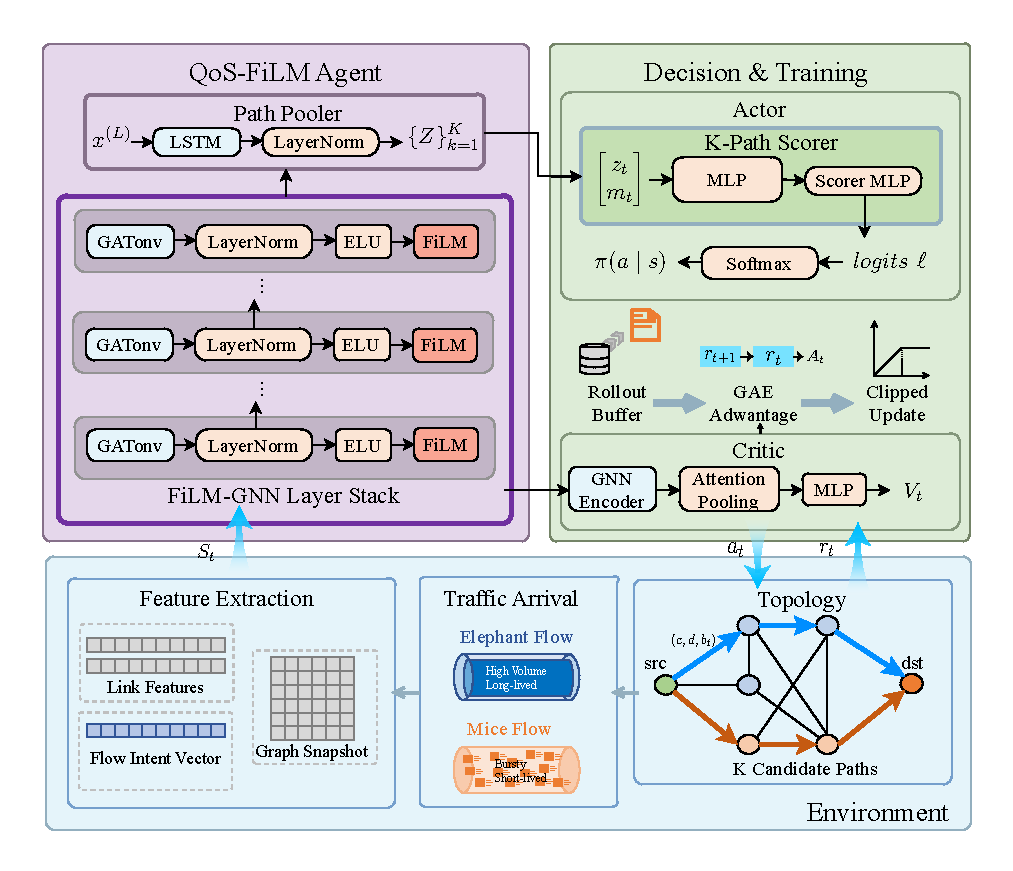
\includegraphics[width=\linewidth]{ENV-REACT.pdf}
\caption{Overall architecture of QoS-FiLM.}
\label{fig:film_gnn_arch}
\end{figure}

\subsection{Problem Formalization: MDP Modeling}
\label{sec:method:mdp}

We formalize the online routing optimization of Section~\ref{sec:problem:objective} as a Markov decision process $(\mathcal{S},\mathcal{A},P,r)$. The agent makes sequential decisions: at step $t$ it selects, for the $t$-th flow $\mathbf{f}_t$, a path from the candidate set $\mathcal{P}_t$.

\textbf{State} $s_t = (\mathcal{G}_t,\, m_t,\, \mathcal{P}_t) \in \mathcal{S}$ consists of three parts:
\begin{enumerate}
\item \emph{Graph snapshot} $\mathcal{G}_t$: node features (marking the source and destination $o_t,v_t$ of the current flow) and link features $[d_e,\,c_e,\,b_e^{\text{res}}]$ (delay, capacity, residual bandwidth);
\item \emph{Flow intent vector} $m_t=[\phi_t,\,\tilde b_t]$, where $\tilde b_t$ is the normalized bandwidth demand;
\item \emph{Candidate paths} $\mathcal{P}_t$ and their validity masks: each path is padded to a fixed tensor length, and the binary mask indicates which positions correspond to actual path nodes versus padding tokens.
\end{enumerate}
The observation contains only the current flow $\mathbf{f}_t$ and excludes future flows $\{\mathbf{f}_\tau\}_{\tau>t}$, consistent with the online causal constraint of Section~\ref{sec:problem:objective}.

\textbf{Action} $a_t\in\mathcal{A}=\{0,1,\dots,K-1\}$ is a discrete choice, selecting the $a_t$-th candidate path $p_t=p_t^{a_t}$ from the $K$ candidates to carry the current flow.

\textbf{Transition} must be distinguished at two levels. Given the current flow and the selected path, \emph{resource accounting is deterministic and known}: the residual bandwidth $b_e^{\text{res}}$ of the links along the path is reduced by $\hat b_t$ (Eq.~\eqref{eq:rho}, the actually allocated bandwidth) and the pointer advances. The next arriving flow $\mathbf{f}_{t+1}$, however, is drawn from the demand distribution $\mathcal{D}$, is invisible to the agent before it arrives, and is unaffected by the current action. The full state transition $P(s_{t+1}\mid s_t,a_t)$ is therefore not deterministic (given $s_t,a_t$, the next state $s_{t+1}$ is not unique); the stochasticity comes from the arrival of the next flow. This matches the ``deterministic accounting, unseen future'' structure described in Section~\ref{sec:problem:objective}.

\textbf{Reward} is taken directly from the utility function $U(\mathbf{f}_t,p_t)$ of Section~\ref{sec:problem:objective} (Eq.~\eqref{eq:utility}), shifted by a constant $-1$ to narrow the reward range and facilitate value function learning:
\begin{equation}
r_t = U(\mathbf{f}_t, p_t) - 1
    = -1 + U^{\text{bw}}_t + U^{\text{dl}}_t.
\label{eq:reward}
\end{equation}
The reward range is $[-1, 1]$. For elephant flows ($\phi_t\to 1$) the delay utility term approaches zero and the reward upper bound is $0$ (attained when $\rho_t=1$); for mouse flows ($\phi_t\to 0$), when bandwidth is fully satisfied and delay is very low, both utility terms can take relatively large positive values, so the reward for this class of flows can exceed $0$. Under a test distribution dominated by mouse flows, the mean reward can therefore be positive overall. Because the offset constant does not change the optimal policy, maximizing the cumulative reward $\sum_t r_t$ is equivalent to maximizing the cumulative utility (Eq.~\eqref{eq:objective}). The structure of Eq.~\eqref{eq:reward} implies that, to earn high rewards on both mouse flows (which require hard bandwidth satisfaction and low latency) and elephant flows (which value the throughput ratio), the policy must \emph{perceive and differentiate the QoS intent} $\phi_t$ of each flow. This motivates the flow-aware encoder presented below.

\subsection{Choice of Training Algorithm}
\label{sec:method:algo}

Section~\ref{sec:problem:objective} argued that this problem is an online stochastic optimization over the demand distribution that requires a non-myopic policy. We adopt PPO as the training algorithm for several reasons: its stochastic policy naturally parameterizes the discrete choice among $K$ candidate paths through a Categorical distribution; its clipped objective keeps updates stable (accommodating the large difference in reward scales between the two flow types); on-policy data collection matches the online deployment setting; combined with generalized advantage estimation (GAE) it achieves the long-range credit assignment that non-myopic decision-making demands; and, being model-free, it does not require explicit modeling of the transition stochasticity caused by the unknown arrival distribution $\mathcal{D}$.

\subsection{Flow-Aware QoS-FiLM Encoder}
\label{sec:method:encoder}

The encoder maps the graph snapshot in the state into node embeddings (i.e., a vector representation for each node). The core idea is that every layer of message passing should ``know which flow is currently being routed,'' so that flows with different QoS intents yield different topological representations. We implement this conditioning with FiLM~\cite{Perez2018_FiLM}. Let the link feature vector be $f_e = [d_e,\, c_e,\, b_e^{\text{res}}] \in \mathbb{R}^3$, the concatenation of delay, capacity, and residual bandwidth.



Let the hidden dimension be $h$. An MLP $\mathrm{MLP}_{\text{lift}}$ first lifts the raw node features to $h$ dimensions: $x^{(0)}=\mathrm{MLP}_{\text{lift}}(x)$. We then stack $L$ graph attention blocks.

The $\ell$-th layer receives the current flow's intent vector $m_t$ and generates per-channel (per-dimension of the $h$-dimensional hidden vector) scaling and shifting parameters through two independent MLPs:
\begin{align}
\gamma^{(\ell)} &= \mathrm{MLP}^{(\ell)}_{\gamma}(m_t), \quad \gamma^{(\ell)}\in\mathbb{R}^{h},
\label{eq:film_gamma}\\
\beta^{(\ell)} &= \mathrm{MLP}^{(\ell)}_{\beta}(m_t), \quad \beta^{(\ell)}\in\mathbb{R}^{h},
\label{eq:film_beta}
\end{align}
and applies FiLM modulation to the message-passing output:
\begin{align}
\tilde x^{(\ell)} &= \mathrm{ELU}\!\big(\mathrm{LN}(\mathrm{Conv}^{(\ell)}(x^{(\ell-1)}, E, f))\big),
\label{eq:conv}\\
x^{(\ell)} &= \big(1+\gamma^{(\ell)}\big)\odot \tilde x^{(\ell)} + \beta^{(\ell)} \;+\; x^{(\ell-1)},
\label{eq:film}
\end{align}
where $\mathrm{Conv}^{(\ell)}$ is a graph attention operator (default: TransformerConv~\cite{Shi2021_UniMP}
% TransformerConv 引用查证:PyTorch Geometric 官方文档及源码(transformer_conv.py)
% 均标注该算子来自 "Masked Label Prediction: Unified Message Passing Model for
% Semi-Supervised Classification"(Shi et al., IJCAI 2021, arXiv:2009.03509),
% 即 Shi2021_UniMP。经三方交叉验证确认此为原始文献。
-style dot-product attention,
with link features $f$ as edge attributes), $\mathrm{LN}$ is layer normalization, $\odot$ is element-wise multiplication, and the final term is a residual connection (adding the layer input directly to its output to ease the training of deep networks). Eq.~\eqref{eq:film} is the key to our method: at \emph{every layer}, the intent vector $m_t$ reshapes node representations through the affine transformation $(1+\gamma)\odot\tilde x+\beta$, so that the same physical topology is encoded into different embeddings for mouse flows and elephant flows. The fundamental distinction from GNN-FiLM~\cite{Brockschmidt2020_GNNFiLM} is the source of $\gamma,\beta$: GNN-FiLM computes them from the \emph{target node representation} to modulate aggregation, whereas we compute them from the \emph{per-flow QoS intent}, making message passing flow-aware.

\subsection{Path Pooling, Scoring, and Value Network}
\label{sec:method:scorer}

\textbf{Path Pooling.} A path pooler (PathPooler) converts the node embeddings $x^{(L)}$ into candidate path representations. For the $k$-th candidate path, the embeddings along its node sequence are extracted to form a variable-length sequence, encoded by an LSTM whose final hidden state is taken, and then passed through layer normalization to yield the path embedding $z_k\in\mathbb{R}^{h}$. The $K$ candidate paths are thus pooled into $\{z_k\}_{k=1}^{K}$.

\textbf{Scoring and Policy.} The scorer $\mathrm{KPathScorer}$ concatenates each path embedding with the current flow intent as $[z_k; m_t]$, passes it through a feature MLP (ELU $+$ LayerNorm) and then a scoring-head MLP, and outputs a scalar logit $\ell_k$ (an unnormalized score). The $K$ logits form a Categorical distribution from which the policy samples an action:
\begin{equation}
\pi_\theta(a_t\!=\!k\mid s_t) = \mathrm{softmax}_k(\ell_1,\dots,\ell_K).
\label{eq:policy}
\end{equation}
If the intent vector $m_t$ entered only at the final scorer, the paths would already have been pooled into fixed vectors, so intent information could no longer back-propagate to influence the topological representation, causing irreversible information loss.

\textbf{Value Network.} The policy and value networks use independent encoders because their optimization objectives conflict: the policy must learn relative preferences among actions to support exploration, whereas the value function must regress scalar returns accurately. Sharing parameters would cause gradient interference and training instability. The value network pools its output node embeddings into a single graph-level vector via attention: each node's attention weight is computed from its embedding and the flow intent $m_t$, so that nodes relevant to the current flow's QoS requirements contribute more to the pooled representation; an MLP regresses this vector into a scalar state value $V_\psi(s_t)$.

\subsection{Training Procedure}
\label{sec:method:train}

Training uses PPO, with advantages computed by GAE. The loss combines the clipped policy objective $\mathcal{L}^{\text{clip}}_\theta$, the value loss $c_v\mathcal{L}^{\text{value}}_\psi$, and the negative entropy bonus $-c_e\mathcal{H}[\pi_\theta]$:
\begin{equation}
\mathcal{L}(\theta,\psi) = \mathcal{L}^{\text{clip}}_\theta + c_v\,\mathcal{L}^{\text{value}}_\psi - c_e\,\mathcal{H}[\pi_\theta],
\label{eq:loss}
\end{equation}
where $\mathcal{L}^{\text{clip}}_\theta$ is the policy objective controlled by the clipping coefficient $\epsilon$, $c_v, c_e$ are value and entropy coefficients respectively, and advantages are normalized within each minibatch. The complete procedure is given in Algorithm~\ref{alg:ppo}.

\begin{algorithm}[t]
\caption{PPO Training for QoS-FiLM}
\label{alg:ppo}
\SetKwInOut{Input}{Input}
\SetKwInOut{Output}{Output}
\Input{Network $G$; demand distribution $\mathcal{D}$; candidate count $K$; sequence length $W$; total frames $T$; batch frames $B$; PPO epochs $E$; learning rate $\eta$}
\Output{Policy parameters $\theta$, value parameters $\psi$}
Randomly initialize $\theta,\psi$\;
\While{collected frames $<T$}{
  \tcp{Collection (on-policy)}
  Interact with environment using current policy $\pi_\theta$ to collect $B$ frames; per step: encode graph $\to$ pool $K$ paths $\to$ score $\to$ sample action via $\pi_\theta$ $\to$ execute routing, deduct bandwidth, record reward $r_t$ (Eq.~\eqref{eq:reward})\;
  \tcp{Advantage estimation}
  Compute advantages $\hat A_t$ and return targets $\hat R_t$ using $V_\psi$ and GAE\;
  \tcp{Optimization}
  \For{$E$ PPO epochs}{
    \ForEach{minibatch}{
      Normalize $\hat A_t$ within minibatch\;
      Compute loss $\mathcal{L}(\theta,\psi)$ (Eq.~\eqref{eq:loss})\;
      Clip gradients, update $\theta,\psi$ with Adam (learning rate $\eta$)\;
    }
  }
  Update learning rate via cosine annealing\;
  \tcp{Evaluation and checkpointing}
  Run several rollouts with deterministic policy, record average reward; save best checkpoint\;
}
\end{algorithm}

\section{Experiments}
\label{sec:exp}

\subsection{Experimental Setup}
\label{sec:exp:setup}

\textbf{Topology and Traffic.} The main experiments are conducted on the GEANT backbone topology ($22$ nodes, $36$ links). To train a policy capable of generalizing across different network states, all link attributes are randomly regenerated at the start of each episode: bandwidth is sampled from $\text{Uniform}[30,100]$ and delay from $\text{Uniform}[1,20]$. Traffic generation uses QoS intent $\phi$ as the dominant variable: $\phi$ is generated from a flipped Pareto distribution ($\alpha\!=\!0.2$), so that the overwhelming majority of flows fall in the low-$\phi$ region (mouse flows with strict bandwidth and delay constraints) and only a small number are high-$\phi$ flows (elephant flows with relaxed constraints). Bandwidth demand $b$ is derived from $\phi$ via a positively correlated linear mapping (Eq.~\eqref{eq:bw_gen}), with $b_{\text{max}}\!=\!40$ and Gaussian noise standard deviation equal to $0.15$ times the span, so that $\phi$ and $b$ remain strongly positively correlated (Pearson $r\!\approx\!0.90$) but not fully deterministic -- $\phi$ still carries independent information beyond $b$.

\textbf{Sequence Length.} Each episode contains $W=150$ flows arriving sequentially, requiring the policy to maintain service quality under long-range credit assignment. Randomized topologies and flow generation ensure that the agent cannot memorize fixed paths and must make differentiated routing decisions based on current link states and the intent of each flow.

\textbf{Baselines.} We compare against four classical routing strategies: OSPF (shortest hop count), ECMP (equal-cost multipath random), CSPF (online constrained shortest path), and RANDOM. All methods are evaluated on the same $200$ test traffic sequences (episodes) and averaged; the PPO policy uses deterministic actions (taking the highest-probability candidate among the $K$ paths, without exploration sampling) to ensure reproducibility.

\textbf{Evaluation Metrics.} Mean Reward (Mean $R$), Bandwidth Satisfaction Score (BW Score, i.e., the mean of per-flow bandwidth satisfaction ratios $\rho_t$), and Average End-to-End Delay (Avg Delay, i.e., the mean of effective delays $\hat D_t$ (Eq.~\eqref{eq:delay}) across all flows). Bandwidth scores are further broken down by flow category (small mouse / mid / big elephant) to examine whether the policy differentiates treatment by QoS intent.

\subsection{Hyperparameters and Implementation Details}
\label{sec:exp:hyperparam}

All hyperparameters denoted symbolically in Sections~\ref{sec:problem}--\ref{sec:method} are assigned specific values in Table~\ref{tab:hyperparam}, with the rationale as follows. For model architecture, the hidden dimension $h=256$ and 4-layer GNN follow the common configuration range of $h\in[64,256]$ and $L\in[2,5]$ seen in RouteNet~\cite{Rusek2020_JSAC_RouteNet} and GNN-FiLM~\cite{Brockschmidt2020_GNNFiLM} in routing scenarios; the single attention head matches the default setting of prior work~\cite{Shi2021_UniMP}. For PPO training, $\gamma=1.0$ is used because the task involves finite-horizon episodes (episodic); the remaining clipping coefficient, GAE parameters, and value coefficient follow the defaults of the original PPO papers~\cite{Schulman2017_PPO,Schulman2016_GAE}; the entropy coefficient $c_e=0.01$ and minibatch size were determined via grid search. For the task, Pareto $\alpha=0.2$ makes the proportion of low-$\phi$ flows exceed 80\%, matching the heavy-tailed characteristics of real traffic reported by measurement studies~\cite{CISCO2023_GlobalTraffic}; the ratio of the flow bandwidth upper bound $b_{\text{max}}=40$ to the link capacity lower bound $30$ means a single flow can create a bottleneck, providing a learning signal for the policy to reserve capacity; the delay normalization constant $\tau=38.3$ is taken as the P25 delay of the GEANT topology. Model architecture and training coefficients are identical across all variants; all variants share the same hyperparameters; link attributes are randomly resampled per episode. Implementation is based on PyTorch, TorchRL, and PyTorch Geometric.

\begin{table}[t]
\centering
\caption{Hyperparameter summary. All variants share these values.}
\label{tab:hyperparam}
\setlength{\tabcolsep}{3pt}
\footnotesize
\begin{tabular}{p{1.6cm}p{3.6cm}p{2.8cm}}
\toprule
Category & Hyperparameter & Value \\
\midrule
\multirow{8}{*}{Model Arch.}
 & Hidden dim $h$              & $256$ \\
 & GNN layers $L$            & $4$ \\
 & Attention heads             & $1$ \\
 & Candidate paths $K$          & $16$ \\
 & $\mathrm{MLP}_{\text{lift}}$ hidden & $[64,128]$, GELU \\
 & Scorer feature MLP         & $[512,512]$, ELU$+$LN \\
 & Scoring head MLP             & $[256,128,64]$, ELU$+$LN \\
 & PathPooler            & Single-layer LSTM \\
\midrule
\multirow{8}{*}{PPO Train.}
 & Discount $\gamma$           & $1.0$ \\
 & GAE $\lambda$          & $0.95$ \\
 & Clipping coeff.\ $\epsilon$     & $0.2$ \\
 & Value coeff.\ $c_v$          & $0.5$ \\
 & Entropy coeff.\ $c_e$            & $0.01$ \\
 & Batch frames $B$            & $3000$ \\
 & PPO epochs $E$ / minibatch & $5$ / $512$ \\
 & Learning rate $\eta$ / optimizer   & $3\times10^{-4}$ / Adam \\
\midrule
\multirow{11}{*}{Task}
 & Topology                  & GEANT ($22$ / $36$) \\
 & Link BW gen.           & $\text{Uniform}[30,100]$ \\
 & Link delay gen.           & $\text{Uniform}[1,20]$ \\
 & Sequence length $W$            & $150$ \\
 & Flow BW upper $b_{\text{max}}$ & $40$ \\
 & Flow BW lower $b_{\text{floor}}$ & $0$ \\
 & $\phi$ dist. Pareto $\alpha$ & $0.2$ \\
 & BW noise $\sigma$      & 6.0 \\
 & Delay norm.\ $\tau$  & $38.3$ (GEANT P25)\\
 & Training frames $T$         & $2\times10^{6}$ \\
 & Gradient clip           & $1.0$ \\
\bottomrule
\end{tabular}
\end{table}

\subsection{Experiment I: Flow-Aware Representations Significantly Outperform Classical Routing Algorithms}
\label{sec:exp:main}

We first compare QoS-FiLM against classical routing algorithms to quantify the advantage of flow-aware representations. To isolate the ``learned policy vs.\ classical algorithm'' comparison, this section contrasts QoS-FiLM against the four classical baselines; ablation comparisons with the noFiLM-Tf and MLP (no message-passing) variants are deferred to Section~\ref{sec:exp:repr}.

At $W\!=\!150$, \textcolor{red}{FiLM-GNN} outperforms all classical baselines on all three metrics of mean reward, bandwidth satisfaction, and delay (Fig.~\ref{fig:main_bars}): its mean reward of $+0.121$ surpasses the strongest classical baseline CSPF ($-0.046$) by $+0.167$, BW Score of $0.759$ exceeds CSPF ($0.473$) by $0.286$, and average delay drops from $130.0$ to $112.9$~ms. Although CSPF has the lowest delay ($125.9$), it does so at the sacrifice of bandwidth satisfaction (BW Score only $0.473$), resulting in the lowest overall reward ($-0.208$)\textcolor{red}{这个值怎么跟本段前面的值不一致？} — looking at delay alone cannot reflect the global trade-off in service quality. This advantage holds across all three topologies (Fig.~\ref{fig:main_bars}): QoS-FiLM outperforms the respective strongest baseline CSPF on GEANT ($+0.121$ vs.\ $-0.046$), NOBEL-EU ($-0.108$ vs.\ $-0.183$), and ABILENE ($+0.122$ vs.\ $+0.041$), demonstrating that the advantage of flow-aware representations is robust across topologies.

\textbf{Source of Advantage: Non-Myopic Long-Range Resource Allocation.} Classical algorithms (including the ``stepwise optimal'' CSPF) make independent greedy routing decisions for each flow and lack awareness of reserving capacity for subsequent flows; under the long sequence length of $W\!=\!150$, early-arriving flows deplete critical link capacity, leaving later flows with no viable path. Bucketing by $\phi$ makes this clear: in the low-intent bucket ($\phi<0.2$, the most strictly constrained mouse flows), \textcolor{red}{FiLM-GNN} achieves a reward of $+0.315$, far surpassing CSPF's $+0.070$; in the mid-intent bucket the two converge; in the high-intent bucket all methods score low — an inherent resource scarcity characteristic of the task. This confirms the argument of Section~\ref{sec:problem:why_rl}: routing is a sequential decision problem with long-range credit assignment, and CSPF, as the representative of ``stepwise optimal,'' is systematically surpassed by the learned non-myopic policy.

\begin{figure*}[t]
\centering
\subimg{p9b_bars_geant_linear_reward.pdf}\hfill
\subimg{p9b_bars_nobel_eu_reward.pdf}\hfill
\subimg{p9b_bars_abilene_reward.pdf}\\[4pt]
\subimg{p9b_bars_geant_linear_bw.pdf}\hfill
\subimg{p9b_bars_nobel_eu_bw.pdf}\hfill
\subimg{p9b_bars_abilene_bw.pdf}\\[4pt]
\subimg{p9b_bars_geant_linear_delay.pdf}\hfill
\subimg{p9b_bars_nobel_eu_delay.pdf}\hfill
\subimg{p9b_bars_abilene_delay.pdf}
\caption{Experiment I: Final performance bar chart comparison across three topologies. (a)--(c) mean reward (mean of 3 seeds, error bars $\pm$ std.\ dev.); (d)--(f) bandwidth service rate; (g)--(i) average delay (ms). Columns from left to right: GEANT ($W\!=\!150$), NOBEL-EU ($W\!=\!150$), ABILENE ($W\!=\!50$). Solid colored bars represent learned network variants (QoS-FiLM highlighted), gray hatched bars represent static baselines.}
\label{fig:main_bars}
\end{figure*}

\subsection{Experiment II: Representational Capacity Ablation -- Message Passing and Intent Conditioning}
\label{sec:exp:repr}

To isolate the contribution of each architectural component, we design three variants along the progressive path of ``no graph structure $\to$ with graph structure but no flow awareness $\to$ with graph structure and flow awareness'' (Fig.~\ref{fig:main_bars}), all sharing the same TransformerConv backbone and hyperparameters, differing only in their representational mechanism:
\begin{itemize}
\item \textbf{MLP} (no message passing): removes message passing, replacing $\mathrm{Conv}$ in Eq.~\eqref{eq:conv} with a per-node MLP (still retaining FiLM modulation), ignoring the edge set $E$ and link features $f$, to test whether graph structure information is necessary.
\item \textbf{noFiLM-Tf} (with message passing but intent only concatenated at the end): removes the $\gamma,\beta$ modulation of Eq.~\eqref{eq:film} (equivalent to $\gamma\equiv 0,\beta\equiv 0$); the intent vector $m_t$ does not enter message passing and is only concatenated with path embeddings at the final scorer, so all flows see the same graph.
\item \textbf{QoS-FiLM} (per-layer intent injection): our method, modulating node representations at every layer via the FiLM affine transformation of Eq.~\eqref{eq:film}.
\end{itemize}

\textbf{Message passing is foundational.} The MLP baseline scores worst on all three metrics (mean reward $-0.177$, BW Score $0.520$), with all flows degenerating into selecting the same path slot (Table~\ref{tab:film_w150_bw} shows converging scores across categories, approximating OSPF-equivalent behavior). Without neighbor aggregation, the model cannot perceive the global distribution of link utilization and cannot differentiate routing for flows with different intents -- confirming that graph structure information is indispensable for routing learning.

\textbf{Per-layer intent injection (FiLM) brings significant gains.} Under the same GNN backbone, per-layer intent-injected QoS-FiLM ($+0.121$) significantly outperforms end-only intent-concatenated noFiLM-Tf ($-0.098$), $\Delta R\!=\!+0.219$; BW Score improves by $+0.158$ ($0.759$ vs.\ $0.601$), and average delay drops from $157.8$ to $112.9$ (a reduction of $44.9$~ms). Fig.~\ref{fig:repr_training} shows the Eval Reward training curves of the two variants. The disadvantage of noFiLM-Tf stems from intent information being concatenated only at the end, unable to apply $\gamma\!\cdot\! x+\beta$ modulation to per-layer node representations, and thus unable to reshape the message-passing process according to flow intent. This trend is consistent across all three topologies (Fig.~\ref{fig:repr_training}): QoS-FiLM clearly leads noFiLM-Tf and MLP, and converges faster with smaller variance (NOBEL-EU: QoS-FiLM $-0.108$ vs.\ noFiLM-Tf $-0.282$; ABILENE: $+0.122$ vs.\ $+0.008$).

\begin{figure*}[t]
\centering
\subimg{p9b_groupA_geant_linear_eval.pdf}\hfill
\subimg{p9b_groupA_nobel_eu_eval.pdf}\hfill
\subimg{p9b_groupA_abilene_eval.pdf}\\[4pt]
\subimg{p9b_groupA_geant_linear_bw.pdf}\hfill
\subimg{p9b_groupA_nobel_eu_bw.pdf}\hfill
\subimg{p9b_groupA_abilene_bw.pdf}
\caption{Experiment II: Training curves of QoS-FiLM, noFiLM-Tf, and MLP on three topologies (mean of 3 seeds $\pm$ std.\ dev.\ confidence band). (a)--(c) Evaluation Reward; (d)--(f) Bandwidth Service Rate. Columns from left to right: GEANT ($W\!=\!150$), NOBEL-EU ($W\!=\!150$), ABILENE ($W\!=\!50$). Gray dashed lines indicate the final evaluation performance of classical baselines.}
\label{fig:repr_training}
\end{figure*}

Viewing by $\phi$ bucket (Table~\ref{tab:film_w150_phi}), QoS-FiLM achieves a delay of only $77.6$ in the latency-sensitive bucket ($\phi<0.2$), a reduction of $68.4$~ms compared to noFiLM-Tf ($146.0$); whereas in the latency-insensitive bucket ($\phi\geq 0.8$), QoS-FiLM's delay ($290.0$) is actually higher than noFiLM-Tf's ($225.9$). This ``low-down, high-up'' pattern is the expected behavior of FiLM conditioning: the policy discriminates among different $\phi$ values and actively transfers delay resources from high-intent flows to low-intent ones, achieving a significant improvement in service quality for the low-intent bucket at minimal cost. By bandwidth category (Table~\ref{tab:film_w150_bw}), QoS-FiLM's BW Score on small flows reaches $0.932$ (noFiLM-Tf only $0.669$, gain $+0.263$), and similarly leads substantially on mid flows ($0.857$ vs.\ $0.614$); on big flows QoS-FiLM is slightly lower ($0.348$ vs.\ $0.483$), but achieves ultra-high scores on small/mid flows at a relatively small cost to big flows, a favorable overall trade-off.

\begin{table}[t]
\centering
\caption{Experiment II ablation -- $\phi$-bucketed delay ($W\!=\!150$, 200 ep $\times$ 3 seeds)\protect\footnotemark[1].}
\label{tab:film_w150_phi}
\setlength{\tabcolsep}{3pt}
\begin{tabular}{lccc}
\toprule
Model & $\phi<0.2$ & $0.2\!\le\!\phi\!<\!0.8$ & $\phi\!\ge\!0.8$ \\
\midrule
\textbf{QoS-FiLM} & $\mathbf{77.6}$ & $190.0$ & $290.0$ \\
noFiLM-Tf        & $146.0$ & $181.7$ & $225.9$ \\
MLP              & $156.3$ & $183.7$ & $220.2$ \\
\bottomrule
\end{tabular}
\end{table}

\begin{table}[t]
\centering
\caption{Experiment II ablation -- BW categories ($W\!=\!150$, 200 ep $\times$ 3 seeds)\protect\footnotemark[1].}
\label{tab:film_w150_bw}
\setlength{\tabcolsep}{3pt}
\begin{tabular}{lccc}
\toprule
Model & $b<8$ & $8\!\le\!b\!<\!32$ & $b\!\ge\!32$ \\
\midrule
\textbf{QoS-FiLM} & $\mathbf{0.932}$ & $\mathbf{0.857}$ & $0.348$ \\
noFiLM-Tf        & $0.669$ & $0.614$ & $0.483$ \\
MLP              & $0.568$ & $0.531$ & $0.431$ \\
\bottomrule
\end{tabular}
\end{table}
\footnotetext[1]{All metrics are the mean summary of 3 random seeds on GEANT (200 ep $\times$ 3 seeds, $W\!=\!150$).\textcolor{red}{不要脚注吧？}}

\subsection{Experiment III: Graph Attention Operator Selection -- TransformerConv vs.\ GATv2Conv}
\label{sec:exp:conv}

We next compare two graph attention operators under the same FiLM framework. TransformerConv uses dot-product attention, while GATv2Conv uses dynamic additive attention~\cite{Brody2022_GATv2}, representing two different attention paradigms. Fig.~\ref{fig:conv_training} shows the training curve comparison of QoS-FiLM under the two operators (along with noFiLM-GATv2 as a reference) across three topologies; QoS-FiLM stably leads FiLM-GATv2 on all three topologies\textcolor{red}{这句话是不是有歧义？}.

\begin{figure*}[t]
\centering
\subimg{p9b_groupB_geant_linear_eval.pdf}\hfill
\subimg{p9b_groupB_nobel_eu_eval.pdf}\hfill
\subimg{p9b_groupB_abilene_eval.pdf}\\[4pt]
\subimg{p9b_groupB_geant_linear_bw.pdf}\hfill
\subimg{p9b_groupB_nobel_eu_bw.pdf}\hfill
\subimg{p9b_groupB_abilene_bw.pdf}
\caption{Experiment III: Training curves of QoS-FiLM, FiLM-GATv2, and noFiLM-GATv2 on three topologies (mean of 3 seeds $\pm$ std.\ dev.\ confidence band). (a)--(c) Evaluation Reward; (d)--(f) Bandwidth Service Rate. Columns from left to right: GEANT ($W\!=\!150$), NOBEL-EU ($W\!=\!150$), ABILENE ($W\!=\!50$).}
\label{fig:conv_training}
\end{figure*}

In terms of final policy quality (Fig.~\ref{fig:conv_training}), QoS-FiLM (TransformerConv$+$FiLM) is optimal in mean reward ($+0.121$) and bandwidth score ($0.759$), substantially leading FiLM-GATv2 ($-0.097$, $0.596$), with a BW Score gap of $+0.163$. The root cause of the performance difference between the two operators lies in their fundamentally different treatment of link attributes (delay, capacity, residual bandwidth $f_e=[d_e,c_e,b_e^{\text{res}}]$). TransformerConv injects link attributes into both the attention key and the message value: attention weight $\alpha_{i,j}=\mathrm{softmax}((\mathbf{W}_3\mathbf{x}_i)^{\top}(\mathbf{W}_4\mathbf{x}_j+\mathbf{W}_6\mathbf{e}_{ij})/\sqrt{d})$, message $\mathbf{W}_2\mathbf{x}_j+\mathbf{W}_6\mathbf{e}_{ij}$. The link feature $\mathbf{e}_{ij}$ independently modulates attention via multiplicative interaction (inner product) -- a high-residual-bandwidth link can receive higher attention weight without depending on target node features; simultaneously, the link feature directly constitutes the message content, so aggregated information naturally carries link quality signals. In contrast, GATv2Conv~\cite{Brody2022_GATv2} mixes link and node features in an additive manner: $\alpha_{i,j}\propto\exp(\mathbf{a}^{\top}\mathrm{LeakyReLU}(\mathbf{\Theta}_s\mathbf{x}_i+\mathbf{\Theta}_t\mathbf{x}_j+\mathbf{\Theta}_e\mathbf{e}_{ij}))$. Link features are summed with source and target node features before jointly entering the nonlinear activation, causing the link quality signal to be strongly coupled with node features -- the attention weight of a high-bandwidth link depends heavily on the neighboring node representations, diluting the independent discriminative power of link attributes. In a routing scenario, link residual bandwidth is a hard constraint signal for path selection and should independently and directly influence neighbor aggregation; TransformerConv's dual-channel injection of link attributes (key + value) naturally suits this need, whereas GATv2Conv's additive mixing weakens the independent expressiveness of link quality.

By $\phi$ bucket (Table~\ref{tab:conv_w150_phi}), QoS-FiLM similarly exhibits the ``low-down, high-up'' pattern described in Section~\ref{sec:exp:repr}: delay in the low-intent bucket is only $77.6$ (GATv2 is $135.2$, a reduction of $57.6$~ms), while delay in the high-intent bucket of $290.0$ is slightly higher than GATv2's $253.5$ -- TransformerConv identifies the $\phi$ semantics of flows more accurately than GATv2, transferring delay resources from high-intent to low-intent flows. By bandwidth category (Table~\ref{tab:conv_w150_bw}), QoS-FiLM's small/mid bandwidth scores ($0.932$/$0.857$) both substantially lead FiLM-GATv2 ($0.667$/$0.618$), with slightly lower big-flow scores ($0.348$ vs.\ $0.456$), achieving ultra-high small/mid flow scores at a relatively small cost to big flows.

\begin{table}[t]
\centering
\caption{Experiment III ablation -- $\phi$-bucketed delay ($W\!=\!150$, 200 ep $\times$ 3 seeds).}
\label{tab:conv_w150_phi}
\setlength{\tabcolsep}{3pt}
\begin{tabular}{lccc}
\toprule
Model & $\phi<0.2$ & $0.2\!\le\!\phi\!<\!0.8$ & $\phi\!\ge\!0.8$ \\
\midrule
\textbf{QoS-FiLM} & $\mathbf{77.6}$ & $190.0$ & $290.0$ \\
FiLM-GATv2       & $135.2$ & $189.1$ & $253.5$ \\
MLP              & $156.3$ & $183.7$ & $220.2$ \\
\bottomrule
\end{tabular}
\end{table}

\begin{table}[t]
\centering
\caption{Experiment III ablation -- BW categories ($W\!=\!150$, 200 ep $\times$ 3 seeds).}
\label{tab:conv_w150_bw}
\setlength{\tabcolsep}{3pt}
\begin{tabular}{lccc}
\toprule
Model & Small BW & Mid BW & Big BW \\
\midrule
\textbf{QoS-FiLM} & $\mathbf{0.932}$ & $\mathbf{0.857}$ & $0.348$ \\
FiLM-GATv2       & $0.667$ & $0.618$ & $0.456$ \\
MLP              & $0.568$ & $0.531$ & $0.431$ \\
\bottomrule
\end{tabular}
\end{table}

\subsubsection{Strong Synergy Between FiLM and Operator: Two-Dimensional Non-Additivity}
\label{sec:exp:synergy}

We further examine whether operator choice and conditioning interact synergistically. We supplement the noFiLM-GATv2 variant, forming a $2\times2$ comparison table of operator $\times$ conditioning (Table~\ref{tab:synergy_2x2})\textcolor{red}{（可以不改，思考一下）MLP有FiLM，但是这个表里没有MLP的结果；是不是能跟noFilM-Tf对比说明图结构和Film哪个更重要？}.

The key finding is: \emph{the gain from FiLM strongly depends on the underlying operator}. On TransformerConv, introducing FiLM brings a massive improvement of $\Delta R\!=\!+0.219$ ($-0.098\!\to\!+0.121$); but on GATv2, the gain from FiLM is merely $\Delta R\!=\!+0.007$ ($-0.104\!\to\!-0.097$), nearly ineffective. This indicates that the two dimensions are not independently additive but exhibit strong synergy: the aforementioned difference in how link attributes are handled amplifies the gap in FiLM effectiveness -- TransformerConv independently injects link attributes into attention keys and message values, providing a high-quality, link-level differentiable representational foundation for FiLM's per-layer intent modulation; whereas GATv2Conv mixes link attributes into node features, so even if FiLM accurately injects flow intent at each layer, the intent signal struggles to be converted into effective path differentiation through the diluted link quality representations. Therefore, the combination of TransformerConv and FiLM is not a simple superposition of two independent advantages, but a synergistic product in which neither can be omitted.

\begin{table}[t]
\centering
\caption{Operator $\times$ conditioning $2\times2$ comparison table (Mean $R$, $W\!=\!150$, 200 ep $\times$ 3 seeds). Values in parentheses show the FiLM gain $\Delta R$ on the same operator.}
\label{tab:synergy_2x2}
\setlength{\tabcolsep}{6pt}
\begin{tabular}{lcc}
\toprule
 & TransformerConv & GATv2Conv \\
\midrule
w FiLM & $\mathbf{+0.121}$ & $-0.097$ \\
w/o FiLM & $-0.098$ & $-0.104$ \\
\midrule
$\Delta R$ (FiLM gain) & $\mathbf{+0.219}$ & $+0.007$ \\
\bottomrule
\end{tabular}
\end{table}

The parameter overhead of FiLM is an operator-independent constant of $+6{,}144$ (relative overhead only $+0.6\%\sim+2.0\%$, coming from two intent$\to$hidden-dim linear layers $\mathrm{MLP}_\gamma,\mathrm{MLP}_\beta$). On the TransformerConv backbone, FiLM trades less than $1\%$ of parameters for an improvement of $\Delta R\!=\!+0.219$, yielding high cost-effectiveness.

\subsection{Experiment IV: Interpretability -- How Flow Intent Influences Representation and Decision}
\label{sec:exp:interp}

To further understand the mechanism of FiLM conditioning, this section examines the essential differences between FiLM and noFiLM-Tf in responding to flow intent from two perspectives: the \emph{representation level} and the \emph{decision level}.

\textbf{Representation level: intent-driven hidden feature sensitivity.} Fixing the network topology and link utilization state, we inject flows with gradually varying QoS intent $\phi$ into the same (src, dst) node pair and observe the hidden features produced by the encoder. We compute intent sensitivity (total change in hidden representations caused by varying $\phi$ under the same state) over $8$ random network states and $\phi\!\in\!\{0.05,0.2,0.5,0.8,0.95\}$: the FiLM encoder has a sensitivity as high as $46.46$, while noFiLM-Tf is only $1.4\times10^{-6}$ (numerically zero), a difference of seven orders of magnitude (Table~\ref{tab:interp_repr}). Furthermore, as $\phi$ gradually increases from the baseline ($0.05\!\to\!0.95$), the drift of FiLM representations monotonically increases ($0\!\to\!8.6\!\to\!25.8\!\to\!40.5\!\to\!46.5$), indicating that intent is smoothly and continuously encoded into node representations; whereas the drift of noFiLM-Tf remains zero throughout. This confirms the ablation design at the architectural level (noFiLM indeed cannot perceive intent) and provides direct quantitative evidence that FiLM injects per-flow intent into node representations. Fig.~\ref{fig:embedding_separation} further shows the PCA projection of hidden features from both encoders: FiLM's representations migrate continuously with $\phi$, while noFiLM-Tf's representations are completely overlapping.

\begin{table}[t]
\centering
\caption{Experiment IV representation level: hidden representation change when only $\phi$ varies under the same network state (GEANT, mean over $8$ states).}
\label{tab:interp_repr}
\setlength{\tabcolsep}{5pt}
\begin{tabular}{lcc}
\toprule
 & Intent Sensitivity & Drift ($\phi\!:0.05\!\to\!0.95$) \\
\midrule
\textbf{QoS-FiLM}  & $\mathbf{46.46}$ & $0\to8.6\to25.8\to40.5\to46.5$ \\
noFiLM-Tf         & $1.4\times10^{-6}$ & All zero \\
\bottomrule
\end{tabular}
\end{table}

\begin{figure*}[t]
\centering
\subimgw{p9b_hidden_diff_film_tf.pdf}\hfill
\subimgw{p9b_hidden_diff_nofilm_tf.pdf}
\caption{Comparison of hidden features for an extreme small flow and an extreme large flow under the same network state and (src, dst) pair.\textcolor{red}{后面的这个子标题直接放到上面的(a)(b)后面} (a) QoS-FiLM; (b) noFiLM-Tf.}
\label{fig:embedding_separation}
\end{figure*}

\textbf{Decision level: intent-driven path selection diversity.} Differences at the representation level ultimately manifest as changes in routing behavior. We compute the entropy of the path-slot selection distribution (in bits; higher indicates more diverse selection, more differentiation by state and intent) for both variants over $200$ test episodes comprising $460$ (src, dst) pairs. FiLM's mean entropy is $2.235$, significantly higher than noFiLM-Tf's $1.962$ (paired $t\!\approx\!14.7$, highly significant\textcolor{red}{这里有t-test，前面V-C里面是不是最好也要有}); on $76\%$ of (src, dst) pairs, FiLM's entropy is higher, and FiLM on average uses $10.4$ path slots while noFiLM-Tf uses only $7.9$. This indicates that the FiLM policy can make finer-grained, more differentiated path selections based on current link states and each flow's intent, whereas noFiLM-Tf, unable to perceive intent, can only rely on state and concentrates its selection on fewer path slots. This comparison corroborates the sensitivity evidence from the representation level: \emph{intent injected into representations by FiLM drives more diverse path selection}, linking representation-level differentiation to decision-level behavior.


\section{Conclusion}
\label{sec:conclusion}

This paper presents QoS-FiLM, a graph neural network architecture that uses per-flow QoS intent as a conditioning signal to address online routing under heterogeneous traffic. QoS-FiLM injects flow intent into every message-passing layer of the GNN through feature-wise linear modulation, so that the same physical topology produces differentiated node embeddings for flows with different QoS requirements, resolving the ``same graph, same embedding'' problem of representational homogeneity. Experiments show that QoS-FiLM outperforms classical baselines in cumulative utility, bandwidth satisfaction ratio, and end-to-end latency across multiple backbone topologies. Ablation studies confirm that per-layer FiLM conditioning yields a performance gain of $+0.219$ over the flow-unaware variant, that the choice of graph attention operator strongly modulates this gain, and that FiLM and the attention operator interact synergistically rather than additively. Interpretability analysis verifies that the FiLM encoder is highly sensitive to QoS intent at the representation level while the flow-unaware baseline cannot perceive intent changes. 
Future work will (i) extend the approach to multi-domain topologies, and adaptive candidate-path generation, and (ii) investigate meta-learning strategies for rapid adaptation to unseen network topologies.


\bibliographystyle{IEEEtran}
\bibliography{related_work}

\end{document}

